\documentclass[12pt,twoside]{article}
\usepackage{amsmath, amssymb}
\usepackage{amsmath}
\usepackage[active]{srcltx}
\usepackage{amssymb}
\usepackage{amscd}
\usepackage{makeidx}
\usepackage{amsthm}
\usepackage{algpseudocode}
\usepackage{algorithm}
\usepackage{listings}
\usepackage{graphicx}
\usepackage{wrapfig}
\usepackage{tikz}
\renewcommand{\baselinestretch}{1}
\setcounter{page}{1}
\setlength{\textheight}{21.6cm}
\setlength{\textwidth}{14cm}
\setlength{\oddsidemargin}{1cm}
\setlength{\evensidemargin}{1cm}
\pagestyle{myheadings}
\thispagestyle{empty}
\markboth{\small{Pr\'actica 7. Eduardo, Daniel.}}{\small{.}}
\date{}
\begin{document}
\centerline{\bf An\'alisis de Algoritmos, Sem: 2020-1, 3CV2, Pr\'actica 7, 09 de Junio de 2020}
\centerline{}
\centerline{}
\begin{center}
\Large{\textsc{Práctica 7: Verificación en tiempo Polinomial.}}
\end{center}
\centerline{}
\centerline{\bf {Mendoza Mart\'inez Eduardo, Aguilar Gonzalez Daniel.}}
\centerline{}
\centerline{Escuela Superior de C\'omputo}
\centerline{Instituto Polit\'ecnico Nacional, M\'exico}
\centerline{$edoomm8@gmail.com, daguilarglz97@gmail.com$}
\newtheorem{Theorem}{\quad Theorem}[section]
\newtheorem{Definition}[Theorem]{\quad Definition}
\newtheorem{Corollary}[Theorem]{\quad Corollary}
\newtheorem{Lemma}[Theorem]{\quad Lemma}
\newtheorem{Example}[Theorem]{\quad Example}
\bigskip
\textbf{Resumen:} La siguiente pr\´actica pretende mostrar la implementación de un algoritmo que nos determine si un ciclo es Hamiltoniano o no asi como su comportamiento, sus tiempos de ejecuci\´on, y la complejidad de este. \newline
{\bf Palabras Clave:} Complejidad P, NP y NPC, Grafo, Ciclo Hamiltoniano.
\section{Introducci\'on}
En la presente práctica se pretende mostrar el desarrollo de un algoritmo el cual tomará como parámetros un grafo y un certificado y este algoritmo verificará si un certificado es un ciclo Hamiltoniano o no del grafo, verificando si lo hace en tiempo polinomial mediante gráficas tomadas durante la ejecución de este algoritmo.

\section{Conceptos B\'asicos}
Es importante conocer algunos de los temas a tratar para la experimentación de la presente práctica. Con buenas bases teóricas, se puede comprender de mucho mejor manera los experimentos a realizar. Por ello, a continuación se presentan algunos conceptos básicos relevantes a la práctica.

\subsection{Complejidad y problemas P (Polinomiales)}
P es la clase de complejidad que contiene problemas de decisión que se pueden resolver en un tiempo polinómico.

Los algortimos de complejidad polinomica se dice que son tratables en el sentido de que suelen ser ejecutados en la practica.
Los problemas que existen para los algoritmos con esta complejidad, se dicen que forman la clase P.
P contiene a la mayoría de problemas naturales, algoritmos de programación lineal, funciones simples,... Por ejemplo la suma de dos números naturales se resuelven en tiempo polinómico (para ser más exactos es de orden 2n). Entre los problemas que se pueden resolver en tiempo polinómico nos encontramos con diversas variedades como los logarítmicos (log(n)), los lineales (n), los cuadráticos (n2), los cúbicos (n3)

 Los problemas de clase "P" son "fáciles" de resolver para los ordenadores; es decir, las soluciones a estos problemas pueden ser calculadas en una cantidad razonable de tiempo, en comparación con la complejidad del problema.

\subsection{Complejidad y Problemas NP (No Polinomiales)}
La clase de complejidad NP contiene problemas que no pueden resolverse en un tiempo polinómico. Cuando se dice que un algoritmo no puede obtener una solución a un problema en tiempo polinómico siempre se intenta buscar otro procedimiento que lo consiga mejorar.

Los problemas de clase NP incluyen muchos problemas de patrones y optimización, que son de gran interés práctico, como por ejemplo la capacidad de determinar la colocación óptima de los transistores en un chip de silicio, el desarrollo de modelos precisos de previsión financiera, o el análisis del comportamiento del pliegue de proteínas en una célula.

Muchos de estos problemas pueden caracterizarse por el hecho de que puede aplicarse a un algoritmo polinómico para ser comprobados sus posibles soluciones, de esta forma se determina si es válida o inválida.
Por medio de esta característica podemos ejecutar un método de resolución no determinista, que consiste en aplicar heurísticos para obtener soluciones hipotéticas que se van desestimando  aceptando al ritmo polinómico.

\subsection{Problemas NP-C (NP - Completos)}
Es el subconjunto de los problemas de decisión en NP tal que todo problema en NP se puede reducir en cada uno de los problemas de NP-completo. Se puede decir que los problemas de NP-completo son los problemas más difíciles de NP y muy probablemente no formen parte de la clase de complejidad P. La razón es que de tenerse una solución polinómica para un problema NP-completo, todos los problemas de NP tendrían también una solución en tiempo polinómico.

Son problemas NP y son los peores problemas posibles de la clase NP, son de extrema complejidad, se caracterizan por ser todas iguales. La teoría NP completo se basa en el concepto de transformación Polinomial.

\subsection{Grafo}
Un grafo es un conjunto, no vacío, de objetos llamados vértices (o nodos) y una selección de pares de vértices, llamados aristas (edges en inglés) que pueden ser orientados o no. Típicamente, un grafo se representa mediante una serie de puntos (los vértices)
conectados por líneas (las aristas).

Un grafo es una pareja de conjuntos $G = (V,A)$,
donde $V$ es el conjunto de vértices, y $A$ es el
conjunto de aristas, este último es un conjunto de
pares de la forma $(u,v)$ tal que $u,v \in V$ . Para
simplificar, notaremos la arista $(a,b)$ como $ab$.
En teoría de grafos, sólo queda lo esencial del
dibujo: la forma de las aristas no son relevantes, sólo
importa a qué vértices están unidas.  La posición de
los vértices tampoco importa, y se puede variar para obtener un dibujo más claro. Muchas redes de uso cotidiano pueden ser modeladas con un grafo: una red de carreteras que conecta ciudades, una red eléctrica o la red de drenaje de una ciudad.

\subsection{Ciclo Hamiltoniano}
Un ciclo es una sucesión de aristas adyacentes,
donde no se recorre dos veces la misma arista, y
donde se regresa al punto inicial. Un ciclo
hamiltoniano tiene además que recorrer todos los
vértices exactamente una vez (excepto el vértice del
que parte y al cual llega).

Un ciclo hamiltoniano es un ciclo que pasa por todos los vértices del grafo. Si el grafo admite un ciclo de estas características, se denomina grafo hamiltoniano.Hoy en día, no se conocen métodos generales para hallar un ciclo hamiltoniano en tiempo polinómico, siendo la
búsqueda por fuerza bruta de todos los posibles caminos u otros métodos excesivamente costosos. Existen, sin
embargo, métodos para descartar la existencia de ciclos o caminos hamiltonianos en grafos pequeños.
El problema de determinar la existencia de ciclos hamiltonianos, entra en el conjunto de los NP-completos
\begin{center}
    \includegraphics[width=5.8cm\textwidth]{hamilton.png}\\
    Figura 1- Ciclo Hamiltoniano
\end{center}

\section{Experimentaci\'on y Resultados}
En esta sección se estudiará el algoritmo para verificar el problema de los ciclos Hamiltonianos, se plantea llegar a un orden de complejidad lineal de este algoritmo para observar que, en efecto, se trata de un problema NP. A su vez, se mostrará su pseudocódigo, funcionamiento y cálculo de complejidad gráfica y analiticamente.

\subsection{Pseudocódigo del algoritmo de verificación hamiltoniana}
Como fue descrito anteriormente, un grafo es una tupla de vertices y aristas y para facilitar las pruebas a realizar, los caminos que se implementaron se consideraron como tuplas, al igual que lo son las aristas. Dado que los caminos serán tuplas (ejemplo: 1-2-3-1 = (1,2),(2,3),(3,1)) se observa que de esta forma en un ciclo simple los vertices serán leidos exactamente 2 veces, esto es importante a consiederar para el funcionamiento del algoritmo propuesto. En seguida, se muestra el pseudocódigo utilizado para este algoritmo.
\begin{lstlisting}
Verificacion_Hamilton(Grafo G, Camino C)
1-  d = diccionario(keys: vertices,
                    values: veces que se recorrio el vertice)
2-  n = |C.recorridos|
3-  for i = 0 to i < n do
4-      if C.recorridos[i] in G.aristas
           or invertir(C.recorridos[i]) in G.aristas do
5-          if C.recorridos[i][0] not in d.keys() do
6-              d[C.recorridos[i][0]] = 1
7-          else if d[C.recorridos[i][0]] == 1 do
8-              d[C.recorridos[i][0]]++
9-          else do
10-             return 0
11-         if C.recorridos[i][1] not in d.keys() do
12-             d[C.recorridos[i][1]] = 1
13-         else if d[C.recorridos[i][1]] == 1 do
14-             d[C.recorridos[i][1]]++
15-         else do
16-             return 0
17-     else do
18-         return 0
19- if |d.keys()| != |G.vertices()| do
20-     return 0
21- m = |d.values()|
22- for i = 0 to i < m do
23-     if d.values()[i] != 2 do
24-         return 0
25- return 1
\end{lstlisting}

\subsection{Cálculo analítico del orden de complejidad}
Por el método de bloques, podemos calcular el orden de complejidad del algoritmo \textit{Verificacion\_Hamilton}. Se definene los bloques como se muestran a continuación.
\\\\
$B_1 =$ Línea 1 a 2\\
$B_2 =$ Línea 3\\
$B_3 =$ Línea 4 a 18\\
$B_4 =$ Línea 19 a 21\\
$B_5 =$ Línea 22\\
$B_6 =$ Línea 23 a 25\\\\
Teniendo esto podemos asignar su respectivo costo computacional, tal como lo vemos en la siguiente tabla.
\begin{center}
    \begin{tabular}{|l|l|}
    \hline
    Bloque & Costo\\
    \hline
    $B_{1}$ &$\Theta(1)$\\
    \hline
    $B_{2}$ & $\Theta(n)$ \\
    \hline
    $B_{3}$ &$\Theta(1)$\\
    \hline
    $B_{4}$ & $\Theta(1)$\\
    \hline
    $B_{5}$ & $\Theta(n)$\\
    \hline
    $B_{6}$ & $\Theta(1)$\\
    \hline
    \end{tabular}
\end{center}
Así entonces, se tiene que,
\begin{center}
    $Verificacion\_Hamilton \in \Theta(1) + \Theta(n) + \Theta(1) + \Theta(1) + \Theta(n) + \Theta(1)$\\\\
    $\therefore Verificacion\_Hamilton \in \Theta(n)$
\end{center}

\subsection{Funcionamiento del algoritmo}
Basandonos en el pseudocódigo propuesto, se implementaron dos clases en Python, la clase \textit{Grafo} con 2 atributos, el primero de ellos es \textit{vertices} (una simple lista donde se almacenan los números de los vertices) y el segundo atributo fue \textit{aristas} (una lista de tuplas). Se sobreescribio el método \textit{str} para una mejor visualización de los grafos y basandonos en un ejemplo dado en las diapositivas obtuvimos lo mostrado en la figura 2.
\begin{center}
    \includegraphics[width=14cm\textwidth]{hamilton/1.png}\\
    Figura 2 - Implementación de la clase \textit{Grafo}
\end{center}
En la figura 3 se tiene la representación gráfica de este grafo.
\begin{center}
    \tikzset{every picture/.style={line width=0.75pt}} %set default line width to 0.75pt
    \begin{tikzpicture}[x=0.75pt,y=0.75pt,yscale=-1,xscale=1]
%uncomment if require: \path (0,477); %set diagram left start at 0, and has height of 477

%Flowchart: Connector [id:dp7976408367872148]
\draw   (150,139.25) .. controls (150,131.38) and (156.38,125) .. (164.25,125) .. controls (172.12,125) and (178.5,131.38) .. (178.5,139.25) .. controls (178.5,147.12) and (172.12,153.5) .. (164.25,153.5) .. controls (156.38,153.5) and (150,147.12) .. (150,139.25) -- cycle ;
%Flowchart: Connector [id:dp2003865779009697]
\draw   (250,64.25) .. controls (250,56.38) and (256.38,50) .. (264.25,50) .. controls (272.12,50) and (278.5,56.38) .. (278.5,64.25) .. controls (278.5,72.12) and (272.12,78.5) .. (264.25,78.5) .. controls (256.38,78.5) and (250,72.12) .. (250,64.25) -- cycle ;
%Flowchart: Connector [id:dp2981264683264355]
\draw   (350,139.25) .. controls (350,131.38) and (356.38,125) .. (364.25,125) .. controls (372.12,125) and (378.5,131.38) .. (378.5,139.25) .. controls (378.5,147.12) and (372.12,153.5) .. (364.25,153.5) .. controls (356.38,153.5) and (350,147.12) .. (350,139.25) -- cycle ;
%Flowchart: Connector [id:dp7486012010103347]
\draw   (300,214.25) .. controls (300,206.38) and (306.38,200) .. (314.25,200) .. controls (322.12,200) and (328.5,206.38) .. (328.5,214.25) .. controls (328.5,222.12) and (322.12,228.5) .. (314.25,228.5) .. controls (306.38,228.5) and (300,222.12) .. (300,214.25) -- cycle ;
%Flowchart: Connector [id:dp434199428421578]
\draw   (200,214.25) .. controls (200,206.38) and (206.38,200) .. (214.25,200) .. controls (222.12,200) and (228.5,206.38) .. (228.5,214.25) .. controls (228.5,222.12) and (222.12,228.5) .. (214.25,228.5) .. controls (206.38,228.5) and (200,222.12) .. (200,214.25) -- cycle ;
%Straight Lines [id:da6275384993291742]
\draw    (164.25,153.5) -- (200,214.25) ;
%Straight Lines [id:da2856704639354024]
\draw    (228.5,214.25) -- (300,214.25) ;
%Straight Lines [id:da23221677105534844]
\draw    (328.5,214.25) -- (364.25,153.5) ;
%Straight Lines [id:da0827982440199242]
\draw    (164.25,125) -- (250,64.25) ;
%Straight Lines [id:da23215157861464641]
\draw    (364.25,125) -- (278.5,64.25) ;
%Straight Lines [id:da7411758290892112]
\draw    (178.5,139.25) -- (350,139.25) ;
%Straight Lines [id:da30526114099857793]
\draw    (214.25,200) -- (264.25,78.5) ;
%Straight Lines [id:da7429323294489873]
\draw    (264.25,78.5) -- (312,198.75) ;

% Text Node
\draw (158.5,130) node [anchor=north west][inner sep=0.75pt]   [align=left] {1};
% Text Node
\draw (258.5,55) node [anchor=north west][inner sep=0.75pt]   [align=left] {2};
% Text Node
\draw (358.5,130) node [anchor=north west][inner sep=0.75pt]   [align=left] {3};
% Text Node
\draw (308.5,205) node [anchor=north west][inner sep=0.75pt]   [align=left] {4};
% Text Node
\draw (208.5,205) node [anchor=north west][inner sep=0.75pt]   [align=left] {5};


\end{tikzpicture}\\
    Figura 3 - Representación gráfica del grafo dado como ejemplo
\end{center}
Posterior a esto, se implemento otra clase denominada \textit{Camino} en donde se tuvo un solo un atributo \textit{recorrido} que funge como una lista de tuplas similar a las \textit{aristas} de \textit{Grafo}. Asimismo, se sobreescribio el método \textit{str} y su funcionamiento se muestra en la figura 4.
\begin{center}
    \includegraphics[width=10cm\textwidth]{hamilton/2.png}\\
    Figura 4 - Implementación de la clase \textit{Camino}
\end{center}
Y una vez teniendo esto, se implementó la función \textit{Verificacion\_Hamilton}, basada en el pseudocódigo previamente colocado. De igual manera, se crearon 3 caminos más para comprobar que su funcionamiento fuera el correcto. En la figura 5 vemos que efectivamente trabaja como debe de hacerlo esta función.
\begin{center}
    \includegraphics[width=9cm\textwidth]{hamilton/3.png}\\
    Figura 5 - Implementación de la función \textit{Verificacion\_Hamilton}
\end{center}
A continuación, se mostrará de manera gráfica el recorrido de todos estos caminos sobre el grafo, de tal modo que se pueda corroborar que esta función cumple su trabajo. \\\\
Para el primer certificado en donde se obtuvo como resultado un $1$ se tuvo lo siguiente
\begin{center}
    Certificado 1: 1-2-3-4-5-1\\\\
    \tikzset{every picture/.style={line width=0.75pt}} %set default line width to 0.75pt
    \begin{tikzpicture}[x=0.75pt,y=0.75pt,yscale=-1,xscale=1]
%uncomment if require: \path (0,477); %set diagram left start at 0, and has height of 477

%Flowchart: Connector [id:dp7976408367872148]
\draw  [color={rgb, 255:red, 74; green, 144; blue, 226 }  ,draw opacity=1 ] (150,139.25) .. controls (150,131.38) and (156.38,125) .. (164.25,125) .. controls (172.12,125) and (178.5,131.38) .. (178.5,139.25) .. controls (178.5,147.12) and (172.12,153.5) .. (164.25,153.5) .. controls (156.38,153.5) and (150,147.12) .. (150,139.25) -- cycle ;
%Flowchart: Connector [id:dp2003865779009697]
\draw  [color={rgb, 255:red, 74; green, 144; blue, 226 }  ,draw opacity=1 ] (250,64.25) .. controls (250,56.38) and (256.38,50) .. (264.25,50) .. controls (272.12,50) and (278.5,56.38) .. (278.5,64.25) .. controls (278.5,72.12) and (272.12,78.5) .. (264.25,78.5) .. controls (256.38,78.5) and (250,72.12) .. (250,64.25) -- cycle ;
%Flowchart: Connector [id:dp2981264683264355]
\draw  [color={rgb, 255:red, 74; green, 144; blue, 226 }  ,draw opacity=1 ] (350,139.25) .. controls (350,131.38) and (356.38,125) .. (364.25,125) .. controls (372.12,125) and (378.5,131.38) .. (378.5,139.25) .. controls (378.5,147.12) and (372.12,153.5) .. (364.25,153.5) .. controls (356.38,153.5) and (350,147.12) .. (350,139.25) -- cycle ;
%Flowchart: Connector [id:dp7486012010103347]
\draw  [color={rgb, 255:red, 74; green, 144; blue, 226 }  ,draw opacity=1 ] (300,214.25) .. controls (300,206.38) and (306.38,200) .. (314.25,200) .. controls (322.12,200) and (328.5,206.38) .. (328.5,214.25) .. controls (328.5,222.12) and (322.12,228.5) .. (314.25,228.5) .. controls (306.38,228.5) and (300,222.12) .. (300,214.25) -- cycle ;
%Flowchart: Connector [id:dp434199428421578]
\draw  [color={rgb, 255:red, 74; green, 144; blue, 226 }  ,draw opacity=1 ] (200,214.25) .. controls (200,206.38) and (206.38,200) .. (214.25,200) .. controls (222.12,200) and (228.5,206.38) .. (228.5,214.25) .. controls (228.5,222.12) and (222.12,228.5) .. (214.25,228.5) .. controls (206.38,228.5) and (200,222.12) .. (200,214.25) -- cycle ;
%Straight Lines [id:da6275384993291742]
\draw [color={rgb, 255:red, 74; green, 144; blue, 226 }  ,draw opacity=1 ]   (164.25,153.5) -- (200,214.25) ;
%Straight Lines [id:da2856704639354024]
\draw [color={rgb, 255:red, 74; green, 144; blue, 226 }  ,draw opacity=1 ]   (228.5,214.25) -- (300,214.25) ;
%Straight Lines [id:da23221677105534844]
\draw [color={rgb, 255:red, 74; green, 144; blue, 226 }  ,draw opacity=1 ]   (328.5,214.25) -- (364.25,153.5) ;
%Straight Lines [id:da0827982440199242]
\draw [color={rgb, 255:red, 74; green, 144; blue, 226 }  ,draw opacity=1 ]   (164.25,125) -- (250,64.25) ;
%Straight Lines [id:da23215157861464641]
\draw [color={rgb, 255:red, 74; green, 144; blue, 226 }  ,draw opacity=1 ]   (364.25,125) -- (278.5,64.25) ;
%Straight Lines [id:da7411758290892112]
\draw    (178.5,139.25) -- (350,139.25) ;
%Straight Lines [id:da30526114099857793]
\draw    (214.25,200) -- (264.25,78.5) ;
%Straight Lines [id:da7429323294489873]
\draw    (264.25,78.5) -- (312,198.75) ;

% Text Node
\draw (158.5,130) node [anchor=north west][inner sep=0.75pt]   [align=left] {1};
% Text Node
\draw (258.5,55) node [anchor=north west][inner sep=0.75pt]   [align=left] {2};
% Text Node
\draw (358.5,130) node [anchor=north west][inner sep=0.75pt]   [align=left] {3};
% Text Node
\draw (308.5,205) node [anchor=north west][inner sep=0.75pt]   [align=left] {4};
% Text Node
\draw (208.5,205) node [anchor=north west][inner sep=0.75pt]   [align=left] {5};


\end{tikzpicture}\\
    Figura 6 - Certificado 1 recorrido sobre el grafo
\end{center}
Mientras que para el segundo certificado en donde se obtuvo un $0$, se observa lo siguiente
\begin{center}
    Certificado 2: 1-2-4-3-5-1\\\\
    \tikzset{every picture/.style={line width=0.75pt}} %set default line width to 0.75pt
    \begin{tikzpicture}[x=0.75pt,y=0.75pt,yscale=-1,xscale=1]
%uncomment if require: \path (0,477); %set diagram left start at 0, and has height of 477

%Flowchart: Connector [id:dp7976408367872148]
\draw  [color={rgb, 255:red, 74; green, 144; blue, 226 }  ,draw opacity=1 ] (150,139.25) .. controls (150,131.38) and (156.38,125) .. (164.25,125) .. controls (172.12,125) and (178.5,131.38) .. (178.5,139.25) .. controls (178.5,147.12) and (172.12,153.5) .. (164.25,153.5) .. controls (156.38,153.5) and (150,147.12) .. (150,139.25) -- cycle ;
%Flowchart: Connector [id:dp2003865779009697]
\draw  [color={rgb, 255:red, 74; green, 144; blue, 226 }  ,draw opacity=1 ] (250,64.25) .. controls (250,56.38) and (256.38,50) .. (264.25,50) .. controls (272.12,50) and (278.5,56.38) .. (278.5,64.25) .. controls (278.5,72.12) and (272.12,78.5) .. (264.25,78.5) .. controls (256.38,78.5) and (250,72.12) .. (250,64.25) -- cycle ;
%Flowchart: Connector [id:dp2981264683264355]
\draw  [color={rgb, 255:red, 74; green, 144; blue, 226 }  ,draw opacity=1 ] (350,139.25) .. controls (350,131.38) and (356.38,125) .. (364.25,125) .. controls (372.12,125) and (378.5,131.38) .. (378.5,139.25) .. controls (378.5,147.12) and (372.12,153.5) .. (364.25,153.5) .. controls (356.38,153.5) and (350,147.12) .. (350,139.25) -- cycle ;
%Flowchart: Connector [id:dp7486012010103347]
\draw  [color={rgb, 255:red, 74; green, 144; blue, 226 }  ,draw opacity=1 ] (300,214.25) .. controls (300,206.38) and (306.38,200) .. (314.25,200) .. controls (322.12,200) and (328.5,206.38) .. (328.5,214.25) .. controls (328.5,222.12) and (322.12,228.5) .. (314.25,228.5) .. controls (306.38,228.5) and (300,222.12) .. (300,214.25) -- cycle ;
%Flowchart: Connector [id:dp434199428421578]
\draw  [color={rgb, 255:red, 208; green, 2; blue, 27 }  ,draw opacity=1 ] (200,214.25) .. controls (200,206.38) and (206.38,200) .. (214.25,200) .. controls (222.12,200) and (228.5,206.38) .. (228.5,214.25) .. controls (228.5,222.12) and (222.12,228.5) .. (214.25,228.5) .. controls (206.38,228.5) and (200,222.12) .. (200,214.25) -- cycle ;
%Straight Lines [id:da6275384993291742]
\draw [color={rgb, 255:red, 208; green, 2; blue, 27 }  ,draw opacity=1 ]   (164.25,153.5) -- (200,214.25) ;
%Straight Lines [id:da2856704639354024]
\draw    (228.5,214.25) -- (300,214.25) ;
%Straight Lines [id:da23221677105534844]
\draw [color={rgb, 255:red, 74; green, 144; blue, 226 }  ,draw opacity=1 ]   (328.5,214.25) -- (364.25,153.5) ;
%Straight Lines [id:da0827982440199242]
\draw [color={rgb, 255:red, 74; green, 144; blue, 226 }  ,draw opacity=1 ]   (164.25,125) -- (250,64.25) ;
%Straight Lines [id:da23215157861464641]
\draw    (364.25,125) -- (278.5,64.25) ;
%Straight Lines [id:da7411758290892112]
\draw    (178.5,139.25) -- (350,139.25) ;
%Straight Lines [id:da30526114099857793]
\draw    (214.25,200) -- (264.25,78.5) ;
%Straight Lines [id:da7429323294489873]
\draw [color={rgb, 255:red, 74; green, 144; blue, 226 }  ,draw opacity=1 ]   (264.25,78.5) -- (312,198.75) ;
%Straight Lines [id:da5713560805057787]
\draw [color={rgb, 255:red, 208; green, 2; blue, 27 }  ,draw opacity=1 ]   (353.5,148.25) -- (226.5,205.25) ;

% Text Node
\draw (158.5,130) node [anchor=north west][inner sep=0.75pt]   [align=left] {1};
% Text Node
\draw (258.5,55) node [anchor=north west][inner sep=0.75pt]   [align=left] {2};
% Text Node
\draw (358.5,130) node [anchor=north west][inner sep=0.75pt]   [align=left] {3};
% Text Node
\draw (308.5,205) node [anchor=north west][inner sep=0.75pt]   [align=left] {4};
% Text Node
\draw (208.5,205) node [anchor=north west][inner sep=0.75pt]   [align=left] {5};


\end{tikzpicture}\\
    Figura 7 - Certificado 2 recorrido sobre el grafo
\end{center}
Luego con el tercer certificado donde se obtiene también un $0$ podemos representarlo gráficamente esto como se muestra en la figura 8.
\begin{center}
    Certificado 1: 1-3-2-4-3-1\\\\
    \tikzset{every picture/.style={line width=0.75pt}} %set default line width to 0.75pt
    \begin{tikzpicture}[x=0.75pt,y=0.75pt,yscale=-1,xscale=1]
%uncomment if require: \path (0,477); %set diagram left start at 0, and has height of 477

%Flowchart: Connector [id:dp7976408367872148]
\draw  [color={rgb, 255:red, 74; green, 144; blue, 226 }  ,draw opacity=1 ] (150,139.25) .. controls (150,131.38) and (156.38,125) .. (164.25,125) .. controls (172.12,125) and (178.5,131.38) .. (178.5,139.25) .. controls (178.5,147.12) and (172.12,153.5) .. (164.25,153.5) .. controls (156.38,153.5) and (150,147.12) .. (150,139.25) -- cycle ;
%Flowchart: Connector [id:dp2003865779009697]
\draw  [color={rgb, 255:red, 74; green, 144; blue, 226 }  ,draw opacity=1 ] (250,64.25) .. controls (250,56.38) and (256.38,50) .. (264.25,50) .. controls (272.12,50) and (278.5,56.38) .. (278.5,64.25) .. controls (278.5,72.12) and (272.12,78.5) .. (264.25,78.5) .. controls (256.38,78.5) and (250,72.12) .. (250,64.25) -- cycle ;
%Flowchart: Connector [id:dp2981264683264355]
\draw  [color={rgb, 255:red, 74; green, 144; blue, 226 }  ,draw opacity=1 ] (350,139.25) .. controls (350,131.38) and (356.38,125) .. (364.25,125) .. controls (372.12,125) and (378.5,131.38) .. (378.5,139.25) .. controls (378.5,147.12) and (372.12,153.5) .. (364.25,153.5) .. controls (356.38,153.5) and (350,147.12) .. (350,139.25) -- cycle ;
%Flowchart: Connector [id:dp7486012010103347]
\draw  [color={rgb, 255:red, 74; green, 144; blue, 226 }  ,draw opacity=1 ] (300,214.25) .. controls (300,206.38) and (306.38,200) .. (314.25,200) .. controls (322.12,200) and (328.5,206.38) .. (328.5,214.25) .. controls (328.5,222.12) and (322.12,228.5) .. (314.25,228.5) .. controls (306.38,228.5) and (300,222.12) .. (300,214.25) -- cycle ;
%Flowchart: Connector [id:dp434199428421578]
\draw   (200,214.25) .. controls (200,206.38) and (206.38,200) .. (214.25,200) .. controls (222.12,200) and (228.5,206.38) .. (228.5,214.25) .. controls (228.5,222.12) and (222.12,228.5) .. (214.25,228.5) .. controls (206.38,228.5) and (200,222.12) .. (200,214.25) -- cycle ;
%Straight Lines [id:da6275384993291742]
\draw    (164.25,153.5) -- (200,214.25) ;
%Straight Lines [id:da2856704639354024]
\draw    (228.5,214.25) -- (300,214.25) ;
%Straight Lines [id:da23221677105534844]
\draw [color={rgb, 255:red, 208; green, 2; blue, 27 }  ,draw opacity=1 ]   (328.5,214.25) -- (366.75,151.5) ;
%Straight Lines [id:da0827982440199242]
\draw    (164.25,125) -- (250,64.25) ;
%Straight Lines [id:da23215157861464641]
\draw [color={rgb, 255:red, 74; green, 144; blue, 226 }  ,draw opacity=1 ]   (364.25,125) -- (278.5,64.25) ;
%Straight Lines [id:da7411758290892112]
\draw [color={rgb, 255:red, 74; green, 144; blue, 226 }  ,draw opacity=1 ]   (178.5,139.25) -- (350,139.25) ;
%Straight Lines [id:da30526114099857793]
\draw    (214.25,200) -- (264.25,78.5) ;
%Straight Lines [id:da7429323294489873]
\draw [color={rgb, 255:red, 74; green, 144; blue, 226 }  ,draw opacity=1 ]   (264.25,78.5) -- (312,198.75) ;
%Flowchart: Connector [id:dp37209630578328046]
\draw  [color={rgb, 255:red, 208; green, 2; blue, 27 }  ,draw opacity=1 ] (352.5,137.25) .. controls (352.5,129.38) and (358.88,123) .. (366.75,123) .. controls (374.62,123) and (381,129.38) .. (381,137.25) .. controls (381,145.12) and (374.62,151.5) .. (366.75,151.5) .. controls (358.88,151.5) and (352.5,145.12) .. (352.5,137.25) -- cycle ;
%Straight Lines [id:da7966820125041973]
\draw [color={rgb, 255:red, 208; green, 2; blue, 27 }  ,draw opacity=1 ]   (180,136.75) -- (352.5,137.25) ;
%Flowchart: Connector [id:dp35503647390683746]
\draw  [color={rgb, 255:red, 208; green, 2; blue, 27 }  ,draw opacity=1 ] (151.5,137.25) .. controls (151.5,129.38) and (157.88,123) .. (165.75,123) .. controls (173.62,123) and (180,129.38) .. (180,137.25) .. controls (180,145.12) and (173.62,151.5) .. (165.75,151.5) .. controls (157.88,151.5) and (151.5,145.12) .. (151.5,137.25) -- cycle ;

% Text Node
\draw (158.5,130) node [anchor=north west][inner sep=0.75pt]   [align=left] {1};
% Text Node
\draw (258.5,55) node [anchor=north west][inner sep=0.75pt]   [align=left] {2};
% Text Node
\draw (358.5,130) node [anchor=north west][inner sep=0.75pt]   [align=left] {3};
% Text Node
\draw (308.5,205) node [anchor=north west][inner sep=0.75pt]   [align=left] {4};
% Text Node
\draw (208.5,205) node [anchor=north west][inner sep=0.75pt]   [align=left] {5};


\end{tikzpicture}\\
    Figura 8 - Certificado 3 recorrido sobre el grafo
\end{center}
Después con el certificado 4 obtuvimos con la función \textit{Verificacion\_Hamilton} un ciclo Hamiltoniano. Esto se observa en la figura 9.

\begin{center}
    Certificado 1: 2-4-3-1-5-2\\\\
    \tikzset{every picture/.style={line width=0.75pt}} %set default line width to 0.75pt
    \begin{tikzpicture}[x=0.75pt,y=0.75pt,yscale=-1,xscale=1]
%uncomment if require: \path (0,477); %set diagram left start at 0, and has height of 477

%Flowchart: Connector [id:dp7976408367872148]
\draw  [color={rgb, 255:red, 74; green, 144; blue, 226 }  ,draw opacity=1 ] (150,139.25) .. controls (150,131.38) and (156.38,125) .. (164.25,125) .. controls (172.12,125) and (178.5,131.38) .. (178.5,139.25) .. controls (178.5,147.12) and (172.12,153.5) .. (164.25,153.5) .. controls (156.38,153.5) and (150,147.12) .. (150,139.25) -- cycle ;
%Flowchart: Connector [id:dp2003865779009697]
\draw  [color={rgb, 255:red, 74; green, 144; blue, 226 }  ,draw opacity=1 ] (250,64.25) .. controls (250,56.38) and (256.38,50) .. (264.25,50) .. controls (272.12,50) and (278.5,56.38) .. (278.5,64.25) .. controls (278.5,72.12) and (272.12,78.5) .. (264.25,78.5) .. controls (256.38,78.5) and (250,72.12) .. (250,64.25) -- cycle ;
%Flowchart: Connector [id:dp2981264683264355]
\draw  [color={rgb, 255:red, 74; green, 144; blue, 226 }  ,draw opacity=1 ] (350,139.25) .. controls (350,131.38) and (356.38,125) .. (364.25,125) .. controls (372.12,125) and (378.5,131.38) .. (378.5,139.25) .. controls (378.5,147.12) and (372.12,153.5) .. (364.25,153.5) .. controls (356.38,153.5) and (350,147.12) .. (350,139.25) -- cycle ;
%Flowchart: Connector [id:dp7486012010103347]
\draw  [color={rgb, 255:red, 74; green, 144; blue, 226 }  ,draw opacity=1 ] (300,214.25) .. controls (300,206.38) and (306.38,200) .. (314.25,200) .. controls (322.12,200) and (328.5,206.38) .. (328.5,214.25) .. controls (328.5,222.12) and (322.12,228.5) .. (314.25,228.5) .. controls (306.38,228.5) and (300,222.12) .. (300,214.25) -- cycle ;
%Flowchart: Connector [id:dp434199428421578]
\draw  [color={rgb, 255:red, 74; green, 144; blue, 226 }  ,draw opacity=1 ] (200,214.25) .. controls (200,206.38) and (206.38,200) .. (214.25,200) .. controls (222.12,200) and (228.5,206.38) .. (228.5,214.25) .. controls (228.5,222.12) and (222.12,228.5) .. (214.25,228.5) .. controls (206.38,228.5) and (200,222.12) .. (200,214.25) -- cycle ;
%Straight Lines [id:da6275384993291742]
\draw [color={rgb, 255:red, 74; green, 144; blue, 226 }  ,draw opacity=1 ]   (164.25,153.5) -- (200,214.25) ;
%Straight Lines [id:da2856704639354024]
\draw    (228.5,214.25) -- (300,214.25) ;
%Straight Lines [id:da23221677105534844]
\draw [color={rgb, 255:red, 74; green, 144; blue, 226 }  ,draw opacity=1 ]   (328.5,214.25) -- (364.25,153.5) ;
%Straight Lines [id:da0827982440199242]
\draw    (164.25,125) -- (250,64.25) ;
%Straight Lines [id:da23215157861464641]
\draw    (364.25,125) -- (278.5,64.25) ;
%Straight Lines [id:da7411758290892112]
\draw [color={rgb, 255:red, 74; green, 144; blue, 226 }  ,draw opacity=1 ]   (178.5,139.25) -- (350,139.25) ;
%Straight Lines [id:da30526114099857793]
\draw [color={rgb, 255:red, 74; green, 144; blue, 226 }  ,draw opacity=1 ]   (214.25,200) -- (264.25,78.5) ;
%Straight Lines [id:da7429323294489873]
\draw [color={rgb, 255:red, 74; green, 144; blue, 226 }  ,draw opacity=1 ]   (264.25,78.5) -- (312,198.75) ;

% Text Node
\draw (158.5,130) node [anchor=north west][inner sep=0.75pt]   [align=left] {1};
% Text Node
\draw (258.5,55) node [anchor=north west][inner sep=0.75pt]   [align=left] {2};
% Text Node
\draw (358.5,130) node [anchor=north west][inner sep=0.75pt]   [align=left] {3};
% Text Node
\draw (308.5,205) node [anchor=north west][inner sep=0.75pt]   [align=left] {4};
% Text Node
\draw (208.5,205) node [anchor=north west][inner sep=0.75pt]   [align=left] {5};


\end{tikzpicture}\\
    Figura 9 - Certificado 4 recorrido sobre el grafo
\end{center}
Y por último se obtuvo nuevamente un ciclo Hamiltoniano tal como lo vemos en la figura 10.
\begin{center}
    Certificado 1: 5-4-3-2-1-5\\
    \tikzset{every picture/.style={line width=0.75pt}} %set default line width to 0.75pt
    \begin{tikzpicture}[x=0.75pt,y=0.75pt,yscale=-1,xscale=1]
%uncomment if require: \path (0,477); %set diagram left start at 0, and has height of 477

%Flowchart: Connector [id:dp7976408367872148]
\draw  [color={rgb, 255:red, 74; green, 144; blue, 226 }  ,draw opacity=1 ] (150,139.25) .. controls (150,131.38) and (156.38,125) .. (164.25,125) .. controls (172.12,125) and (178.5,131.38) .. (178.5,139.25) .. controls (178.5,147.12) and (172.12,153.5) .. (164.25,153.5) .. controls (156.38,153.5) and (150,147.12) .. (150,139.25) -- cycle ;
%Flowchart: Connector [id:dp2003865779009697]
\draw  [color={rgb, 255:red, 74; green, 144; blue, 226 }  ,draw opacity=1 ] (250,64.25) .. controls (250,56.38) and (256.38,50) .. (264.25,50) .. controls (272.12,50) and (278.5,56.38) .. (278.5,64.25) .. controls (278.5,72.12) and (272.12,78.5) .. (264.25,78.5) .. controls (256.38,78.5) and (250,72.12) .. (250,64.25) -- cycle ;
%Flowchart: Connector [id:dp2981264683264355]
\draw  [color={rgb, 255:red, 74; green, 144; blue, 226 }  ,draw opacity=1 ] (350,139.25) .. controls (350,131.38) and (356.38,125) .. (364.25,125) .. controls (372.12,125) and (378.5,131.38) .. (378.5,139.25) .. controls (378.5,147.12) and (372.12,153.5) .. (364.25,153.5) .. controls (356.38,153.5) and (350,147.12) .. (350,139.25) -- cycle ;
%Flowchart: Connector [id:dp7486012010103347]
\draw  [color={rgb, 255:red, 74; green, 144; blue, 226 }  ,draw opacity=1 ] (300,214.25) .. controls (300,206.38) and (306.38,200) .. (314.25,200) .. controls (322.12,200) and (328.5,206.38) .. (328.5,214.25) .. controls (328.5,222.12) and (322.12,228.5) .. (314.25,228.5) .. controls (306.38,228.5) and (300,222.12) .. (300,214.25) -- cycle ;
%Flowchart: Connector [id:dp434199428421578]
\draw  [color={rgb, 255:red, 74; green, 144; blue, 226 }  ,draw opacity=1 ] (200,214.25) .. controls (200,206.38) and (206.38,200) .. (214.25,200) .. controls (222.12,200) and (228.5,206.38) .. (228.5,214.25) .. controls (228.5,222.12) and (222.12,228.5) .. (214.25,228.5) .. controls (206.38,228.5) and (200,222.12) .. (200,214.25) -- cycle ;
%Straight Lines [id:da6275384993291742]
\draw [color={rgb, 255:red, 74; green, 144; blue, 226 }  ,draw opacity=1 ]   (164.25,153.5) -- (200,214.25) ;
%Straight Lines [id:da2856704639354024]
\draw [color={rgb, 255:red, 74; green, 144; blue, 226 }  ,draw opacity=1 ]   (228.5,214.25) -- (300,214.25) ;
%Straight Lines [id:da23221677105534844]
\draw [color={rgb, 255:red, 74; green, 144; blue, 226 }  ,draw opacity=1 ]   (328.5,214.25) -- (364.25,153.5) ;
%Straight Lines [id:da0827982440199242]
\draw [color={rgb, 255:red, 74; green, 144; blue, 226 }  ,draw opacity=1 ]   (164.25,125) -- (250,64.25) ;
%Straight Lines [id:da23215157861464641]
\draw [color={rgb, 255:red, 74; green, 144; blue, 226 }  ,draw opacity=1 ]   (364.25,125) -- (278.5,64.25) ;
%Straight Lines [id:da7411758290892112]
\draw    (178.5,139.25) -- (350,139.25) ;
%Straight Lines [id:da30526114099857793]
\draw    (214.25,200) -- (264.25,78.5) ;
%Straight Lines [id:da7429323294489873]
\draw    (264.25,78.5) -- (312,198.75) ;

% Text Node
\draw (158.5,130) node [anchor=north west][inner sep=0.75pt]   [align=left] {1};
% Text Node
\draw (258.5,55) node [anchor=north west][inner sep=0.75pt]   [align=left] {2};
% Text Node
\draw (358.5,130) node [anchor=north west][inner sep=0.75pt]   [align=left] {3};
% Text Node
\draw (308.5,205) node [anchor=north west][inner sep=0.75pt]   [align=left] {4};
% Text Node
\draw (208.5,205) node [anchor=north west][inner sep=0.75pt]   [align=left] {5};


\end{tikzpicture}\\
    Figura 10 - Certificado 5 recorrido sobre el grafo
\end{center}

\subsection{Cálculo del orden de complejidad mediante gráficas}
Ya obtenido el orden de complejidad de manera analítica procederemos a determinar el orden de complejidad mediante gráficas obtenidas en las pruebas que se fueron realizando incrementando el número de vertices y aristas que tiene cada grafo respecto al tiempo que tarda en  ejecutarse. Para cada grafo introducido al algoritmo también se introdujeron 3 certificados es decir 3 ciclos los cuales el algoritmo debe verificar si estos ciclos son hamiltonianos o no por lo cual el algoritmo devolvera un 1 si lo son y un 0 si no lo son.\\\\
Como primer prueba comenzamos a calcular los ciclos de los grafos de 3 hasta 7 nodos mostrando su información de cada uno. \\\\
En la figura 11 se muestran 3 grafos uno de 5 vertices y 8 aristas, 6 vertices y 10 aristas y 7 vertices y 12 aristas, de los cuales se muestra el numero de vertices y sus aristas que los componen asi como los 3 ciclo que le corresponden a cada uno. Se muestra cada ciclo y en caso de no ser ciclo hamiltoniano regresa un 0 y el motivo por el cual no cumple las caracteristicas es decir no existe una arista o se repite un vertice etc. En caso de ser un ciclo hamiltoniano regresa un 1 y el tiempo que se tardo en verificar ese ciclo. \\\\
En la figura 12 se muestra la gráfica que se obtuvo despues de ejecutar el algoritmo mostrando el tiempo que tardo en verificar los ciclos de cada grafo.\\\\
\begin{center}
    \includegraphics[width=9cm\textwidth]{hamilton/graficas/7c.png}\\
    Figura 11 - Cálculo Grafos hasta 7 vertices
\end{center}
\begin{center}
    \includegraphics[width=9cm\textwidth]{hamilton/graficas/7g.png}\\
    Figura 12 - Grafica de 7 vertices
\end{center}

Al observar la figura anterior nos damos cuenta que requerimos de más pruebas para encontrar un mejor comportamiento de la grafica asi que haremos una segunda prueba.\\\\
Para una segunda prueba agregaremos 4 grafos más hasta llegar a un grafo con 11 vertices y 20 aristas, los cuales podremos observar en la figura 13. En esta figura solo se muestra el grafo y sus componentes así como el unico camino hamiloniano encontrado en cada uno de ellos y el tiempo que tardó en verificarlo para poder graficarlo asi como se muestra en la figura 14.
\begin{center}
    \includegraphics[width=9cm\textwidth]{hamilton/graficas/11c.png}\\
    Figura 13 - Cálculo Grafos hasta 11 vertices
\end{center}
\begin{center}
    \includegraphics[width=9cm\textwidth]{hamilton/graficas/11g.png}\\
    Figura 14 - Grafica de 11 vertices
\end{center}
Gracias a la figura anterior vemos que la grafica parece tomar una forma lineal por lo que realizaremos una ultima prueba con grafo de 15 vertices y 28 aristas para observar más claramente el comportamiento de la gráfica como se muestra en la figura 16. En la figura 15 mostramos el ciclo hamiltoniano del grafo, sus componentes y el tiempo que tardo en verificar el ciclo.
\begin{center}
    \includegraphics[width=9cm\textwidth]{hamilton/graficas/15c.png}\\
    Figura 15 - Cálculo Grafos de 15 vertices
\end{center}
\begin{center}
    \includegraphics[width=9cm\textwidth]{hamilton/graficas/15g.png}\\
    Figura 16 - Grafica de 15 vertices
\end{center}
Con la figura anterior observamos más claramente como la gráfica comienza a tomar una forma lineal así que lo siguiente es encontrar una función que acote por arriba a nuestra gráfica. La función nos queda de la siguiente forma:
\begin{center}
    $f(n) = \frac{1}{50000}(n)$
\end{center}
En la figura 18 se muestra la gráfica y la función propuesta y en la figura 17 el ciclo de cada grafo y su tiempo de ejecución asi como sus componentes.
\begin{center}
    \includegraphics[width=9cm\textwidth]{hamilton/graficas/15cotac.png}\\
    Figura 17 - Cálculo Grafos hasta 15 verticesa acotada por $f(n)$
\end{center}
\begin{center}
    \includegraphics[width=9cm\textwidth]{hamilton/graficas/15cotag.png}\\
    Figura 18 - Grafica de 15 vertices acotada por $f(n)$
\end{center}
En la figura anterior podemor ver como nuestra función acota de manera correcta nuestra gráfica obtenida con grafos de 3 hasta 15 vertices.\\
Concluyendo asi que graficamente el algoritmo Verificacion Hamilton tiene complejidad de orden Lineal $\theta{(n)}$

\newpage
\section{Conclusiones}
Eduardo Mendoza Martínez\newline
\begin{wrapfigure}{r}{0.5\textwidth}
  \begin{center}
    
\includegraphics[width=6cm\textwidth]{ed.png}
  \end{center}

\end{wrapfigure}
Esta última práctica concluyó de una adecuada forma el curso de Análisis de Algoritmos, en virtud de conocer el tipo de problemáticas que en un futuro podamos enfrentarnos nosotros como próximos ingenieros. Conocer que tipo de problemática es la que se tiene y saberla categorizar entre un problema P, NP o NP-Completo, nos puede permitir estudiar de una mejor manera los algoritmos que lleguemos a realizar, y entre los problemas P, saber calcular \textit{a priori} y \textit{a posteriori} los ordenes de complejidad de los problemas y con ello se puede incluso mejorar algunos algoritmos que tienen ordenes de complejidad no óptimos para solucionar un problema en un tiempo considerablemente corto, tal fue el caso como lo llegamos a ver con el algoritmo de Karatsuba que reduce el tiempo de complejidad para el cálculo de una multiplicación entre 2 números muy grandes y que después se observó de igual forma un algoritmo un tanto similar para de igual forma reducir el tiempo de complejidad del cálculo de multiplicación de matrices con Strassen. U otro ejemplo con el algoritmo de Fibonacci, que en clase vimos el algoritmo clásico de Fibonacci con recursividad que toma complejidad exponencial, mientras que más adelante con programación dinámica obtuvimos tiempos lineales de complejidad del algoritmo de Fibonacci. En lo que respecta a la presente práctica no fue complicada en cuestión, a pesar de tratarse de un problema NP-C, y no fue díficil porque nuestra tarea era quedarnos con la parte NP y demostrar que efectivamente se trata de un problema NP verificándolo a través de un algoritmo con tiempo de complejidad polinomial. Fue distinto definitivamente, graficar los tiempos de este algoritmo de verificación, ya que siempre se habían manejado arreglos con elementos aleatorios en prácticas pasadas para obtener los tiempos de resolución de nuestros algoritmos y en esta última práctica, no podían ser tan arbitrarios los datos ingresados, ya que se usó una estructura que utilizamos por primera vez que fueron los "grafos" y dentro de las listas que se usaron para verificar los ciclos Hamiltonianos se tuvo que colocar entre ellas la solución al problema.
\newline \newline \newline \newline
Daniel Aguilar Gonzalez\newline

En esta última práctica mencionamos la clasificación de los problemas computacionales, P, NP y NP-Completos y como el tiempo en que se ejecutan permite que se clasifiquen de esta manera.

\begin{wrapfigure}{r}{0.5\textwidth}
  \begin{center}
    \includegraphics[width=6cm\textwidth]{dan.png}
\end{center}
\end{wrapfigure}
El saber que clasificación tiene un problema nos permite saber a lo que nos enfrentamos y saber de que manera podemos atacarlo para darle solución, de igual manera nos permite saber un poco qué tipo de recursos requeriremos para su solución.
El tiempo es el que determina si un algoritmo es polinomial o no polinomial como ejemplo de esto es algoritmo presentado anteriormente que verifica si un certificado es un ciclo hamiltoniano o no. El problema de encontrar un ciclo hamiltoniano en un grafo arbitrario se sabe que es NP-C, es decir es uno de los problemas más dificiles de la clasificación NP, pero el verificar si un certificado es ciclo hamiltoniano de un grafo es relativamente sencillo que puede ser resuelto en un tiempo polinomial clasificandose así como problema P.
En esta práctica trabajamos una estructura que personalmente no había trabajado mucho como son "grafos", como declarar sus elementos y el como dentro de ellos pueden haber ciclos que determinan si un grafo pertenece a una clasificación o no. En este caso introducimos 3 certificados es decir 3 ciclos de los cuales 1 de ellos debía ser un ciclo hamiltoniano, para esto se implemento un algoritmo el cual es capáz de determinar esto devolviendo un 0 en caso de que no fuera un ciclo y 1 en caso de serlo. Gracias a esta información determinamos si un grafo es hamiltoniano porque contiene un ciclo hamiltoniano inclusive más de uno. \\
Este curso de análisis de algoritmos me fue sumamente útil ya que pude reforzar algunos conocimientos que ya tenia y aprender otros que desconocía. Aprendí métodos para poder atacar un problema, ventajas y desventajas, dentro de ellos habia algunos que contenian otros para desempeñar correctamente su función. Calcular el orden de complejidad de cada algoritmo fue de vital importancia ya que asi podiamos calcular funciones que acotaran nuestras graficas y así poder  ver si se resolvian en tiempo polinomial o no.

\newpage
\section{Anexo}
En  esta  seccíon  veremos  alguna información o problemas extra de los ya presentados en la práctica.

\subsection{Formula booleana a FNC}
En esta sección presentaremos el algoritmo para poder llegar a la Forma Normal Conjuntiva a partir de una formula.
Antes de comenzar debemos dejar en claro qué es la Forma Normal Conjuntiva. \\
Una fórmula está en forma normal conjuntiva (FNC) si es una conjunción de disyunciones de literales; es decir, es de la forma: \\
\begin{center}
$(L_{1,1} \vee \cdot \cdot \cdot \vee L_{1,n1}) \wedge \cdot \cdot \cdot  \wedge (L_{m,1} \vee \cdot \cdot \cdot \vee L_{m,nm})$
\end{center}
Algoritmo: \\\\
Aplicando a una fórmula F los siguientes pasos se obtiene una forma normal conjuntiva de F, FNC(F):
\begin{itemize}
    \item[1.] Eliminar los bicondicionales usando la equivalencia \newline
		$A \leftrightarrow B \equiv (A \rightarrow B) \wedge (B \rightarrow A)$ \hspace{80}   (1)
	\item[2.] Eliminar los condicionales usando la equivalencia \newline
		$A \rightarrow B \equiv \neg A \vee B$ \hspace{145}   (2)
	\item[3.] Interiorizar las negaciones usando las equivalencias \newline
		$\neg(A \wedge B) \equiv \neg A \vee \neg B$ \hspace{125}   (3)  \newline
		$\neg(A \vee B) \equiv \neg A \wedge \neg B$ \hspace{125}   (4)  \newline
		$\neg\neg A \equiv A$ \hspace{188}   (5)
	\item[4.] Interiorizar las disyunciones usando las equivalencias \newline
		$A \vee (B \wedge C) \equiv (A \vee B) \wedge (A \vee C)$ \hspace{65}   (6) \\
		$(A \wedge B) \vee C \equiv (A \vee C) \wedge (B \vee C)$ \hspace{65}   (7)
\end{itemize}
\subsubsection{Ejemplo}
Ejemplo de cálculo de una FNC de $\neg(p \wedge (q \rightarrow r))$: \\
\begin{cent}

$\neg(p \wedge (q \rightarrow r))$ \\
$\equiv \neg(p \wedge (\neg q \vee r)) $ \hspace{65}  [por (2)]\\
$\equiv \neg p \vee \neg(\neg q \vee r)$ \hspace{66}  [por (3)]\\
$\equiv \neg p \vee (\neg \neg q \wedge \neg r)$ \hspace{58}  [por (4)]\\
$\equiv \neg p \vee (q \wedge \neg r)$
\hspace{74} [por (5)]\\
$\equiv (\neg p \vee q) \wedge (\neg p \vee \neg r)$
\hspace{38}  [por (6)]\\
\end{cent}

\begin{center}
    FNC (F) = $(\neg p \vee q) \wedge (\neg p \vee \neg r)$
\end{center}
\newpage
\section{Bibliograf\'ia}
[1.] A. Jiménez, "P versus NP. ¿Nunca lo entendiste?", Xatakaciencia.com, 2020. [Online]. Available: https://www.xatakaciencia.com/matematicas/p-versus-np-nunca-lo-entendiste.
\newline\newline
[2.] Rodriguezz, "Las clases P NP y NP completo", Es.slideshare.net, 2020. [Online]. Available: https://es.slideshare.net/YlSfSl/las-clases-p-np-y-np-\\completo#:~:text=Los%20problemas%20para%20los%20que,Turing%20determinista%20es%20llamada%20P.
\newline\newline
[3.] "NP-completo", Es.wikipedia.org, 2020. [Online]. Available: https://es.\\wikipedia.org/wiki/NP-completo#:~:text=En%20teor%C3%ADa%20de%20la%20complejidad,los%20problemas%20de%20NP%2Dcompleto.
\newline\newline
[4.] Unipamplona.edu.co, 2020. [Online]. Available: http://www.unipamplo\\na.edu.co/unipamplona/portalIG/home_23/recursos/general/11072012/\\grafo3.pdf. \newline\newline
[5.] Uoc.gitlab.io, 2020. [Online]. Available: http://uoc.gitlab.io/2010/mate\\maticas/modulo%208.%20grafos%20eulerianos%20y%20hamiltanianos.pdf.
\newline\newline
[6.] "LI2011: Formas normales conjuntivas y disyuntivas | Vestigium", Glc.\\us.es, 2020. [Online]. Available:https://www.glc.us.es/~jalonso/vestigium/\\li2011-formales-normales-conjuntivas-y-disyuntivas/.
\end{document}
